\paragraph{Methodology of the \BATA\ subproject.}

In a first round of experiments we will excite resonantly the S$\leftrightarrow$P transition of {\bf Ba$^+$ ions generated by an electrical discharge} between two barium electrodes and will collect the fluorescence signal of the P$\rightarrow$D transition. Although this generation method is not ideal because several different species other than Ba ions will be generated (e.g., BaO molecules or clusters), it does not need a major technological development. 

\begin{figure}
\begin{center}
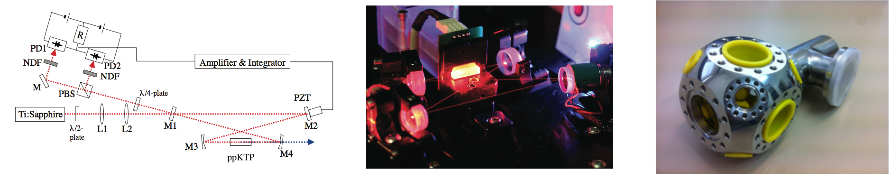
\includegraphics[width=0.99\textwidth]{img/blueLaser.png}
%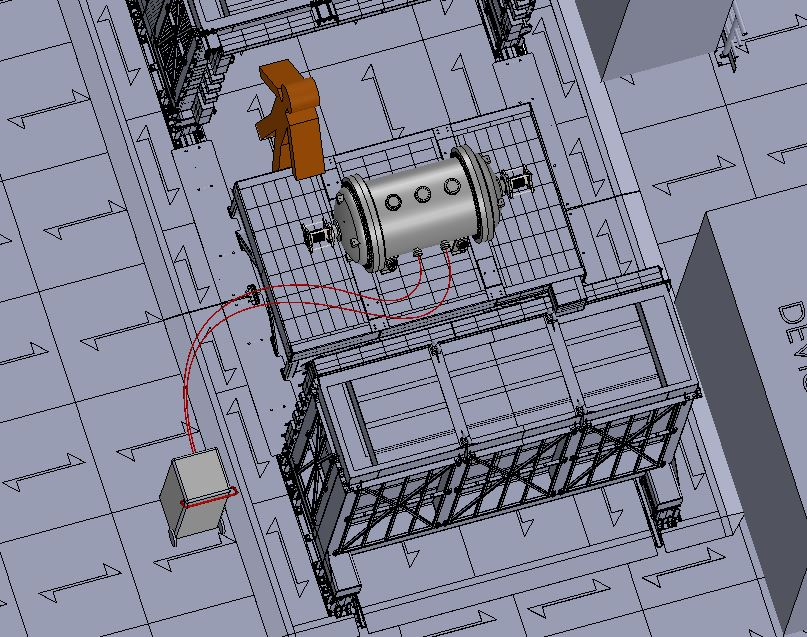
\includegraphics{img/CALIB_LSC_sources.jpg}
\caption{\small Left: experimental set-up for resonant frequency doubling of a 
Ti:Sapphire laser using ppKTP. Right: the chamber for the proof-of-concept experiments, built at IFIC, and ready to be installed at CLPU.}
\label{fig:chamber}
\end{center}
\end{figure}

The laser source needed to resonantly excite the $Ba^{+}$ ions must have a wavelength of 493.5\,nm, not available in commercial lasers. The laser source will therefore be produced at the CLPU, optimising a tunable Ti:sapphire laser at 987\,nm to obtain a second harmonic generation (SHG) at 493.5\,nm, see Figure \ref{fig:chamber}. This setup allows the tuning of the wavelength and the control of the bandwidth of the laser, a necessary feature to precisely tune it to the transition frequency (e.g. to correct for pressure broadening and other effects). The IFIC group, on the other hand, has fabricated the test chamber needed for the experiments (see Fig.~\ref{fig:chamber}). 

It is expected that this initial set of experiments will provide valuable information about the population dynamics in Ba$^+$ ions, and the influence of the different homogeneous and inhomogeneous broadening mechanisms. 

The second objective of the \BATA\ subproject is to {\bf generate Ba ions by an ion source}. For this objective, in order to get a better approximation of the final conditions of NEXT experiment a source of ions will be designed and constructed at the CLPU. This ion source will be based on selective ionisation and mass spectrometry techniques, and it will allow an efficient selection of the desired target species (e.g, $Ba^{+}$~and $Ba^{++}$). With this setup we will be able to study the recombination process Ba$^{++}\rightarrow$Ba$^{+}$ and decide whether it can be induced by collisions with xenon atoms, or whether it requires an additive (see discussion in the objectives of the CALREC subproject). Depending on the results of the experiment, a magnetic trap can be added to improve the experimental conditions. 

The third objective of the \BATA\ subproject is to perform a proof of principle experiment with an {\bf additional laser for deshelving the D state}. Our approach will be to use a second laser to induce a two photon transition (one photon is forbidden by selection rules, between the states D and S, see Fig.\,\ref{fig.BATA}). 	

The fourth objective of the \BATA\ subproject is the {\bf development of a state-of-the-art 4.1\,$\mu$m laser}. There are only a few laser systems that generate laser emission in the mid-infrared (MIR, from 2 to 10\,$\mu$m). There are lasers that emit in discrete wavelengths as gas lasers ($CO_2$, Xe-HE, He-Ne), chemical lasers (Hydrogen Fluoride, Deuterium Fluoride) and Dye lasers by Raman Shift. All these systems are large and complex, emit in relative low power and involve the use of dangerous materials (chemicals, flammable gases and/or carcinogenic powders). 

\begin{figure}[h!]
\begin{center}
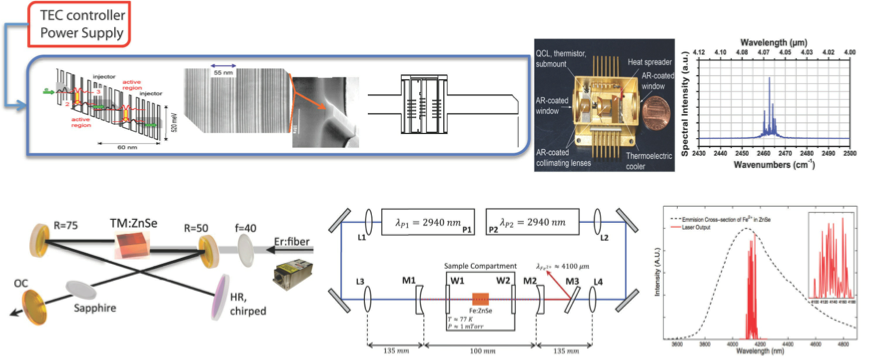
\includegraphics[width=0.99\textwidth]{img/MIR.png}
\end{center}
\caption{\label{Fig:MIR}\small Top: band theory of a quantum cascade laser (QCL), semiconductor material with physical bands and first device with laser spectrum at MIR. Bottom: schematic view of the TM:ZnSe laser design (two potential configurations with Er pumping laser) with potential tunable laser curve and free running emission. All MIR optics are made of CaF2, ZnSe and AR-coated at 2940 - 5000 nm.}
\end{figure}

A much more interesting alternative to reach the desired MIR wavelength is the use of an optically pumped solid state laser (OPSSL) system, by means of a specific doping of crystals with metal transition ions, see Fig.~\ref{Fig:MIR}. Wavelengths of 2 and 2.9\,$\mu$m are available with $Tm^{3+}$, $Tm^{3+}$-$Ho^{3+}$ and $Er^{3+}$ active ions in crystalline matrices. Recent developments involve doping with $Cr^{2+}$ and $Fe^{2+}$ ions. This approach should allow us to develop a laser system that emits in a broad range: 2.1 to 3\,$\mu$m and 3.7 to 5\,$\mu$m, respectively. Another option is to work with quantum cascade semiconductor systems potentially available from 3.8 to 9.5\,$\mu$m in a discrete range, i. e.  not only continuously. 

To develop a laser system around 4.1\,$\mu$m we need to study and evaluate the best optical parameters of some materials (crystalline matrices or semiconductors) that can be used as active laser materials.  This will allow us to design a laser cavity with the appropriate  optical components and devices (these should work in the MIR region). It will also allow us to maximise the efficiency of the laser system. The cavities are different for optically pumped systems (the case of crystals doped with $Cr^{2+}$ o $Fe^{2+}$) or for electrically pumped systems (as the quantum cascade semiconductors). These cavities can be 2-, 3- or 4- folded mirror configurations depending on the advantages observed during the design using optical and numerical software. The characterisation of the laser emission and other related parameters will allow us  to improve the laser system to use in the NEXT experiment. 